\documentclass{article}

% If you're new to LaTeX, here are some short tutorials:
% https://www.overleaf.com/learn/latex/Learn_LaTeX_in_30_minutes
% https://en.wikibooks.org/wiki/LaTeX/Basics

% Formatting
\usepackage[utf8]{inputenc}
\usepackage[margin=1in]{geometry}
\usepackage[titletoc,title]{appendix}

% Math
% https://www.overleaf.com/learn/latex/Mathematical_expressions
% https://en.wikibooks.org/wiki/LaTeX/Mathematics
\usepackage{amsmath,amsfonts,amssymb,mathtools}

% Images
% https://www.overleaf.com/learn/latex/Inserting_Images
% https://en.wikibooks.org/wiki/LaTeX/Floats,_Figures_and_Captions
\usepackage{graphicx,float}

% Tables
% https://www.overleaf.com/learn/latex/Tables
% https://en.wikibooks.org/wiki/LaTeX/Tables

% Algorithms
% https://www.overleaf.com/learn/latex/algorithms
% https://en.wikibooks.org/wiki/LaTeX/Algorithms
\usepackage{algorithm}
\usepackage{algpseudocode}

% References
% https://www.overleaf.com/learn/latex/Bibliography_management_in_LaTeX
% https://en.wikibooks.org/wiki/LaTeX/Bibliography_Management
\usepackage{biblatex}
\addbibresource{references.bib}
\usepackage{tikz}
\usetikzlibrary{calc}
\usepackage{tikz}
\usetikzlibrary{shapes.geometric}
\usepackage{booktabs}

% Title content
\title{Monte Carlo in Monte Carlo, Pathway to Victory in UNO}
\author{Wenyang Hui, Mengyun Liu, Chibin Zhang}
\date{December 31, 2020}

\DefineBibliographyStrings{english}
   {andothers = \mkbibemph{et al\adddot}}
\begin{document}

\maketitle

\newcommand{\todo}[1]{\textbf{\color{red}{todo[#1]}}}

\begin{abstract}

The game UNO, whose name originated from the Latin "One," has simple rules that could be quickly mastered by a three-year-old. But make no mistake, deeply concealed in the simplicity of rules is the combinatoric complexity of game states. The easy to learn but hard to master characteristic of this game makes it an exciting target for artificial intelligence research. In this paper, we create novel adaptations to Monte Carlo Tree Search, a popular game search technique mostly applied in board games, and tailor it to UNO's highly stochastic nature and complex state space. To reflect on what we have learned in class, we also apply strategies such as informed search, expectimax search, and reinforcement learning in our greedy agent, expectimax agent, and deep Q-learning (DQN) agent. We evaluate the effectiveness of our agents by letting them compete against random agents and among themselves. Our experimental result suggests that our Monte-Carlo Tree Search - Hidden Markov Model (MCTS-HMM) agent surpasses the random agent significantly and beats state-of-the-art UNO agent\cite{olivia2020winning} by a wide margin.

\end{abstract}

\section{Introduction}
The game UNO comes in 2 flavors: official or common. Often distributed with a box of UNO cards is a folded sheet of rules of UNO\cite{mattel}. The official rulebook is point-oriented, meaning that for a player to win, he would have to score points and the first person to score 500 points wins the game. Keeping track of points while enjoying the game is indeed a cumbersome task. In reality, when folks play UNO, they seldom refer to the rulebook and instead play by the assumed common rules\cite{wiki:uno}. Common-flavored UNO game plays much similar to a shedding-type card game, i.e., the first player that discards all his hand cards is the winner.

Besides drawing or playing a card, some rules require players to act upon certain events, e.g., calling out "UNO" when playing the next-to-last-card or challenge a player when he plays the "Wild +4" card. Such rules are added for variety and interactivity, but modeling them in a program complicates implementation and analyses. For the sake of clarity, we do not consider them as a valid action for our agent. 



\subsection{Deck}
A regular UNO Deck consists of 108 cards. Judging by the color, a card could be red, yellow, green, blue, or "Wild", in this case, often colored black. Judging from how they influence gameplay, the cards can be either numbered or functional. Numbered cards, when played, is only discarded. Functional cards, on the other hand, have special purposes like forcing the opponent to draw a card that can be used to the user's advantage. A complete listing and count of each card is given in the following table\ref{tab:card}.

\begin{table}[htbp]
    \centering
    \begin{tabular}{ l c }
    \toprule
    Type & Count \\\hline
    Number 0  & $1 \times 4$ \\
    Number 1 - 9   &  $2 \times 4$ \\
    Reverse & $2 \times 4$ \\
    Skip & $2 \times 4$ \\ 
    Draw 2 & $2 \times 4$ \\
    Wild & 8 \\ 
    Wild +4 & 8 \\
    \bottomrule
    \end{tabular}
    \caption{Types of card in UNO and their respective count}
    \label{tab:card}
\end{table}

\subsection{Game Mechanics}
Given the vast array of actions, sources of uncertainty, and our project's limited timespan, we decided to simplify UNO's mechanics. To do so, we made several simplifying assumptions. The exact game rule is shown in the following.

\begin{itemize}
    \item Round start \\
        Flip the card on top of the draw deck. If a non-numbered card appears, put it into the discard pile. Repeat until a numbered card appears. Start the game clockwise with the dealer.
    \item Play \\
        A player could choose to play or draw a card. When he plays a card, his choice must have the same color or the same number as the previous one, or it could be a wild card. A "Reverse" card reverses the direction of the game, e.g., clockwise to counterclockwise. A "Skip" card skips the next opponent's turn. A "+2" card adds 2 cards from the deck to the next opponent's hand and skips his turn.  A "Wild" card is wild in the sense that it can succeed any cards. A "Wild +4" card is similar to the prior, except that it adds 4 cards to the next opponent and skips his turn. If a player has no card to play, then he must keep drawing from the deck until a valid successor appears, or he is satisfied, whichever comes first.
    \item Winning Condition \\
        The first player to discard all his cards is declared victorious
\end{itemize}

\subsection{Difficulty}
\todo{}
\subsection{Contribution}
In this paper, we explore game search techniques taught in class in a real-world setting and dig into the nitty-gritty details of implementing an agent for games with vast imperfect information and huge state space. To the best of our knowledge, we're the first to use Monte-Carlo Tree Search together with Hidden Markov Models to solve the card game UNO. Finally, Our experimental results complement class knowledge by providing a side by side, quantitative, and thorough evaluation of different agents. 


\section{Related Work}
\citeauthor{mnih2015human} showed how reinforcement learning help agents excel in retro video games on the Atari platform. Their evaluation reports the DQN agent performing at a super-human level in 29 out of 49 games, a promising result that largely contributed to the proliferation of reinforcement learning both inside and outside academia. Their monumental achievements greatly motivated and spurred the authors to work on the game search topic. 

\citeauthor{chaslot2010monte}  coined the term Monte-Carlo Tree Search in his Ph.D. thesis, which later gained tremendous popularity in the artificial intelligence research community. He demonstrated his method's effectiveness on a once deemed impossible AI puzzle, go, achieving dan master on a constrained 9 by 9 go board. This same technique was later adopted by Deepmind, conceiving the nowadays household name AlphaGo. While Go is a board game and UNO is a card game, a striking similarity that they both share is the simplicity of rules and the complexity of states. We believe employing MCTS to the UNO scene will be beneficial.

Games and reinforcement learning have long been a research genera in artificial intelligence; nevertheless, few have investigated the effectiveness and practicability of such an approach in UNO until very recently. \citeauthor{zha2019rlcard} designed a collective reinforcement learning framework for common card games, called RLCards. We appreciate and utilize their work to our advantage. Specifically, their implementation of UNO provides insufficient information such as \todo{} that is crucial to decision making of our \todo{} agent. We build upon their library and make changes to expose necessary visible game states to our agent. \citeauthor{olivia2020winning} released their work on a UNO DQN agent. We cite experimental results from their paper and use them as a metric for testing our method's effectiveness.


\section{Methodology}
\subsection{MCTS-HMM Agent}
To \textit{explore}, or to \textit{exploit}, that is the question. As the computational resource is ultimately bounded, a common trade-off that tree search algorithms face is choosing to go deeper or wider. Going deeper means that we could arrive at the terminal state, have full certainty of the outcome, but at the cost of landing on a suboptimal option. Going in breadth let us explore comprehensively, in exchange for limited depth. We don't miss out on the optimal option if there are any, but we would have approximate utilities for the states we've seen so far. Traditional game search strategy like Minimax search requires exploring the shallower layers before proceeding to the deeper layers, even when used together with alpha-beta pruning, resulting in poor performance in real-world problems. On the other hand, MCTS quantitatively unifies exploration and exploitation through the Upper Confidence Bound formula\ref{equ:ucb}, and strike a balance between the two via iterative expansion and simulation. In the following subsections, we explain how MCTS works and the adaptations we made to work on UNO.

\subsubsection{MCTS}
In essence, MCTS can be divided into 4 distinctive phases: selection, expansion, simulation, and back-propagation. In the selection phase, the MCTS algorithm traverses the tree from the root node selecting the node that evaluates the highest UCB value. The UCB formula is given in equation\ref{equ:ucb}, where $x_i$ is the expected utility for state $i$, C is a constant controlling exploration, $t$ is the total simulations, and $n_i$ is the number of times state $i$ was visited.  Due to the frame and scope of this paper, we do not offer a complete derivation of this formula but instead, give an intuition. A closer inspection, the UCB formula resembles the exploration function of Q-learning where the expected value of a state is added to some constant times the inverse of the times the state is visited. When $n_i$ is small, the uncertainty of a given state is large, resulting in a large $S_i$ value, making it more likely to be selected by the agent. When $x_i$ is large, this means that the node's expected utility is high; exploiting the action that transits into this state will likely give good results, so it is also scored with high value. The exact choice as to which state is to be selected made by the agent is influenced by both of the two terms. In the expansion phase, children of the selected node are added to the tree, broadening the fringe. In the simulation phase, the MCTS algorithm goes deep down the tree sampling value from actual terminal states. The sampled value is then propagated back up to the root to improve the accuracy of approximation of the intermediate node's value. After running enough iterations of the aforementioned 4 phases, we gain enough confidence in the optimality of certain actions and take. 

\begin{equation}
    S_i = x_i + C\sqrt{\frac{\ln{t}}{n_i}}
    \label{equ:ucb}
\end{equation}


\subsubsection{Card guessing using HMM}
Although we believe that MCTS is the right direction to take when tackling UNO, an issue that we stumble across is that it does take care of uncertainty. We draw inspiration from Hidden Markov Models (HMM), and Particle filtering algorithm learned from class to overcome this obstacle. Assuming that the prior distribution of each players' cards follows from the uniform, as time goes on, whenever a player plays a card, we update the posterior by observing the cards they've played. This gives us the observation model in equation\ref{equ:obs}. If he instead draws a card, it is sensible to assume that he is sampling from the difference set of the initial deck and the discard pile, which gives us the transition model\ref{equ:tran}. Because exact inference is computationally intensive, we use the particle filtering algorithm for approximation. To elaborate on our implementation in details, each card is assigned \todo{} particles, \todo{} in total in the beginning. Each time a player plays a card, we check if it agrees with our approximation and assign higher weights to particles that do and lower ones that don't. We keep track of the discard pile and apply the transition model when a player draws a card. The weighted particles are resampled each round. Passage of time causes the particles to gather around the highly probable cards, and our opponent model becomes more accurate. We select the most probable cards as input for MCTS queries. In other words, we \textit{determinize} the most likely explanation as a point estimate to deal with UNO's uncertainties.


The transition model opponent's cards
\begin{equation}
    T(x_i|x_{i-1}) = ...
    \label{equ:tran}
\end{equation}

The observation model of opponents's cards
\begin{equation}
    O(x_i|e_{1:i}) = ...
    \label{equ:obs}
\end{equation}

\subsection{Other Agents}
\subsubsection{DQN Agent}

Recall what we have learned about reinforcement learning in class. To solve a model-free MDP problem, we would have to specify the Transition function $T(s, a, s')$ and the Reward function $R(s, a, s)$. Such an approach worked well in limited and constrained setting the like \textit{Gridworld} where the number states never exceeded a hundred and viable actions at each state are within 4. However, the vanilla Q-learning algorithm does not scale to real-world problems. It immediately falls apart in the setting of UNO where states explode to the magnitude of \todo{No. Of states}. Precise representation of state and action pairs would exhaust memory very quickly, even in today's supercomputers, making it intractable both in time and space. 

A popular technique used in combination with reinforcement learning to cope with the state explosion problem is to use a deep neural network as function approximators for q-values. An intuition for such an approach is that while the \todo{} states are indeed unique, most of them only differ by only small variation. A neural network will hopefully capture the similarity between states, generalize, and densely represent experience compared to pure enumeration. In a nutshell, we trade loss of accuracy for computational efficiency.

We adopt such a technique in our DQN agent. A subtlety that arises from providing inputs to the neural network is that neural networks expect fixed-length input while the number of cards in an agent's hand can vary. We solve this problem by converting the list of cards into a fix-sized array of card counts. For instance, if the agent has a "Red 1" and a "Wild" card in hand, [1, 53] is turned into [0, 1, ..., [53] = 1, 0]. Our neural network layer is a \todo{layer} network with \todo{hidden layers}, \todo{} inputs and \todo{} outputs. The input fed into this network is the state viewed from the agent's perspective: 2-tuple of cards in hand and previously played card. This tuple is serialized as a vector and forwarded to the neural network to obtain the approximated q-value. We trained our DQN agent for \todo{} iterations, and average loss over time is depicted in the \ref{fig:loss} below. We visually observe that the loss curve flattens out after about \todo{} iterations, and any further training will unlikely yield substantial improvement, halting the training right there.

Our loss function is given as \ref{equ:loss}
\begin{equation}
    L(\theta) = ...
    \label{equ:loss}
\end{equation}

We observe the loss curve of the DQN agent converges after \todo{} iterations. 
\begin{figure}
    \begin{center}
    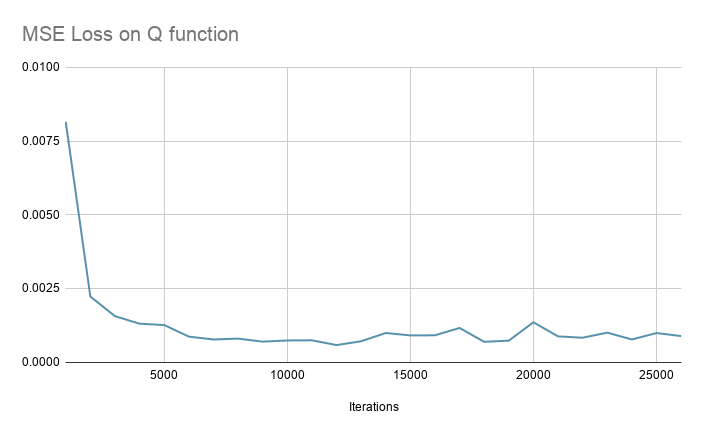
\includegraphics[width=8cm]{MSE Loss on Q function.png}
    \end{center}
    \label{fig:loss}
\end{figure}


\subsubsection{Expectimax Agent}
Expectimax search, as opposed to Minimax Search, is a game search strategy that models opponents acting suboptimally or their action based on chance. In our case, little does the agent know about his opponents: what cards do they hold in their hand? Nor does he have any clue of his environment: what is the next card to be drawn from the deck? Our expectimax agent always assumes that his opponents are random agents; that is, they are equally likely to play or draw a card. More formally, the card played by opponents and cards drawn from the deck follows a uniform distribution. We've tried many utility/evaluation functions and settled on one that worked best empirically. It is so complex describing it would take up a whole section. The following equation is the evaluation function in its most distilled form:
\begin{equation}
    E(s) = ...
\end{equation}


\subsubsection{Greedy Agent}
On a high-level, the greedy agent's strategy is to mimic what a human player would do: greedily minimize the number of cards in hand. It tends to play a card rather than draw a card. In fact, it only chooses to draw as a last resort. When there are multiple cards in hand, it prefers playing numbered cards against functional cards. The fewer cards it has in hand, the less probable it is going to have a card match in color or number with the previous card; saving a "Wild" card appears to be a good strategy. Implementation wise, valid actions are sorted in order of numbered cards, utility cards, and draw. The greedy agent always chooses the first viable action. 

\section{Evaluation}
We evaluate the effectiveness of the 4 agents by performing 2 types of tournaments. In the first tournament, the player count is set to 4, and the selected agent will play against 3 random agents. We record and the number of times each agent wins and divide by the total number of rounds played to get the win rate. In the second tournament, we focus on the pairwise relative strength of agents and let them play in 1 vs. 1 matches.
\subsection{Against Random Agents}
As shown in table \ref{tab:rand}, all agents outperform the random agent, but with a varying degree of significance. Comming in the bottom of the list is the expectimax agent with a win rate of \todo{}. We initially expected the expectimax agent to be at least better than the greedy agent because the implementation is much more complicated (\todo{90 vs. 10 loc}). We attribute its marginal improvement to its limited tree traversal depth and high uncertainty of the game. Once again to our surprise, the greedy agent is almost on par with the DQN agent. Our prior anticipation was that the DQN agent would be the second, if not the best, as we put lots of thought process and validation into it, and it is practiced by other researchers. As mentioned in the previous section, the greedy agent implements a policy close to how human players play the game. Such heuristic, though very simple, deemed very useful. \todo{} The MCTS-HMM agent won a staggering \todo{x out of y round}, but it is also the most computationally intensive one. 
\begin{table}[htbp]
    \centering
    \begin{tabular}{l c c c}
    \toprule
        Number of random agents & 1 & 2 & 3 \\\hline
        MCTS-HMM & 0.96 & 0.95 & 0.94 \\
        DQN & 0.95 & 0.91 & 0.91 \\
        Greedy & 0.95 & 0.91 & 0.89 \\
        Expectimax & N/A & & \\
    \bottomrule
    \end{tabular}
    \caption{Win rate against random agents (1000 rounds) }
    \label{tab:rand}
\end{table}


\subsection{Against one another}
While competing against random agents give us a ranking of the agents, in real life, we seldom judge a player's strength by how well he played against a jerk. Thus we put the agents 1 vs. 1 matches to gain a clearer picture. The results\ref{tab:mat} is in line with table \ref{tab:rand}. Relative strength against random agents implies having the upper hand in an 1 vs 1 match. 

\begin{table}
    \centering
    \begin{tabular}{l c c c c c}
    \toprule
        & MCTS-HMM & DQN & Greedy & Expectimax & Random \\\hline
        MCTS-HMM & 0.55 & 0.55 & 0.6 & N/A & 0.96 \\
        DQN & & & & & \\ 
        Greedy & & 0.46 & N/A & 0.95 \\ 
        Expectimax & & & & & \\ 
        Random \\
    \bottomrule
    \end{tabular}
    \caption{Win rate in 1 vs. 1 matches (1000 rounds)}
    \label{tab:mat}
\end{table}


\subsection{Human interaction}
Due to the limited number of samples, we do not give the win rate of each agent when played against a human player because a win count of 3 out of five carries little statistical significance. However, we do note some of the interesting features of each agent observed during gameplay to give a rough idea of their respective strategy. \todo{} Some plays aggressively, some tends to play defensively, others favor a particular type of move; we think this is primarily due to \todo{}


\section{Conclusion}
In this paper, we make the following contributions. We provide a comprehensive comparison of game playing techniques taught in class, put in real-world settings. We novelly adapt MCTS, which is usually employed in deterministic and fully observable games, to UNO, a game with complex state space and largely imperfect information viewed from the agent's perspective. We believe our determinization technique is generic and practical enough to serve as a general framework to think about card games and real-world problems where partially observable states are the norm. 

\subsection{Future Work}
MCTS runs slowly. Better network structure. Other proposed methods.


% References
\newpage
\printbibliography

\end{document}
